% Options for packages loaded elsewhere
\PassOptionsToPackage{unicode}{hyperref}
\PassOptionsToPackage{hyphens}{url}
%
\documentclass[
  english,
  man]{apa6}
\usepackage{lmodern}
\usepackage{amssymb,amsmath}
\usepackage{ifxetex,ifluatex}
\ifnum 0\ifxetex 1\fi\ifluatex 1\fi=0 % if pdftex
  \usepackage[T1]{fontenc}
  \usepackage[utf8]{inputenc}
  \usepackage{textcomp} % provide euro and other symbols
\else % if luatex or xetex
  \usepackage{unicode-math}
  \defaultfontfeatures{Scale=MatchLowercase}
  \defaultfontfeatures[\rmfamily]{Ligatures=TeX,Scale=1}
\fi
% Use upquote if available, for straight quotes in verbatim environments
\IfFileExists{upquote.sty}{\usepackage{upquote}}{}
\IfFileExists{microtype.sty}{% use microtype if available
  \usepackage[]{microtype}
  \UseMicrotypeSet[protrusion]{basicmath} % disable protrusion for tt fonts
}{}
\makeatletter
\@ifundefined{KOMAClassName}{% if non-KOMA class
  \IfFileExists{parskip.sty}{%
    \usepackage{parskip}
  }{% else
    \setlength{\parindent}{0pt}
    \setlength{\parskip}{6pt plus 2pt minus 1pt}}
}{% if KOMA class
  \KOMAoptions{parskip=half}}
\makeatother
\usepackage{xcolor}
\IfFileExists{xurl.sty}{\usepackage{xurl}}{} % add URL line breaks if available
\IfFileExists{bookmark.sty}{\usepackage{bookmark}}{\usepackage{hyperref}}
\hypersetup{
  pdftitle={Developmental consistency in children's drawings of object categories},
  pdflang={en-EN},
  pdfkeywords={children's drawings, visual production, tracing, object recognition, visuomotor control},
  hidelinks,
  pdfcreator={LaTeX via pandoc}}
\urlstyle{same} % disable monospaced font for URLs
\usepackage{graphicx,grffile}
\makeatletter
\def\maxwidth{\ifdim\Gin@nat@width>\linewidth\linewidth\else\Gin@nat@width\fi}
\def\maxheight{\ifdim\Gin@nat@height>\textheight\textheight\else\Gin@nat@height\fi}
\makeatother
% Scale images if necessary, so that they will not overflow the page
% margins by default, and it is still possible to overwrite the defaults
% using explicit options in \includegraphics[width, height, ...]{}
\setkeys{Gin}{width=\maxwidth,height=\maxheight,keepaspectratio}
% Set default figure placement to htbp
\makeatletter
\def\fps@figure{htbp}
\makeatother
\setlength{\emergencystretch}{3em} % prevent overfull lines
\providecommand{\tightlist}{%
  \setlength{\itemsep}{0pt}\setlength{\parskip}{0pt}}
\setcounter{secnumdepth}{-\maxdimen} % remove section numbering
% Make \paragraph and \subparagraph free-standing
\ifx\paragraph\undefined\else
  \let\oldparagraph\paragraph
  \renewcommand{\paragraph}[1]{\oldparagraph{#1}\mbox{}}
\fi
\ifx\subparagraph\undefined\else
  \let\oldsubparagraph\subparagraph
  \renewcommand{\subparagraph}[1]{\oldsubparagraph{#1}\mbox{}}
\fi
% Manuscript styling
\usepackage{upgreek}
\captionsetup{font=singlespacing,justification=justified}

% Table formatting
\usepackage{longtable}
\usepackage{lscape}
% \usepackage[counterclockwise]{rotating}   % Landscape page setup for large tables
\usepackage{multirow}		% Table styling
\usepackage{tabularx}		% Control Column width
\usepackage[flushleft]{threeparttable}	% Allows for three part tables with a specified notes section
\usepackage{threeparttablex}            % Lets threeparttable work with longtable

% Create new environments so endfloat can handle them
% \newenvironment{ltable}
%   {\begin{landscape}\begin{center}\begin{threeparttable}}
%   {\end{threeparttable}\end{center}\end{landscape}}
\newenvironment{lltable}{\begin{landscape}\begin{center}\begin{ThreePartTable}}{\end{ThreePartTable}\end{center}\end{landscape}}

% Enables adjusting longtable caption width to table width
% Solution found at http://golatex.de/longtable-mit-caption-so-breit-wie-die-tabelle-t15767.html
\makeatletter
\newcommand\LastLTentrywidth{1em}
\newlength\longtablewidth
\setlength{\longtablewidth}{1in}
\newcommand{\getlongtablewidth}{\begingroup \ifcsname LT@\roman{LT@tables}\endcsname \global\longtablewidth=0pt \renewcommand{\LT@entry}[2]{\global\advance\longtablewidth by ##2\relax\gdef\LastLTentrywidth{##2}}\@nameuse{LT@\roman{LT@tables}} \fi \endgroup}

% \setlength{\parindent}{0.5in}
% \setlength{\parskip}{0pt plus 0pt minus 0pt}

% \usepackage{etoolbox}
\makeatletter
\patchcmd{\HyOrg@maketitle}
  {\section{\normalfont\normalsize\abstractname}}
  {\section*{\normalfont\normalsize\abstractname}}
  {}{\typeout{Failed to patch abstract.}}
\makeatother
\shorttitle{Development of drawing}
\author{Bria Long\textsuperscript{1}, Ying Wang\textsuperscript{2}, Stella Christie\textsuperscript{2}, Michael C. Frank\textsuperscript{1}, \& Judith E. Fan\textsuperscript{3}}
\affiliation{
\vspace{0.5cm}
\textsuperscript{1} Stanford University\\\textsuperscript{2} Tsinghua University\\\textsuperscript{3} University of California, San Diego}
\authornote{

Correspondence concerning this article should be addressed to Bria Long, 450 Jane Stanford Way, Stanford CA 94305. E-mail: bria@stanford.edu}
\keywords{children's drawings, visual production, tracing, object recognition, visuomotor control\newline\indent Word count: X}
\DeclareDelayedFloatFlavor{ThreePartTable}{table}
\DeclareDelayedFloatFlavor{lltable}{table}
\DeclareDelayedFloatFlavor*{longtable}{table}
\makeatletter
\renewcommand{\efloat@iwrite}[1]{\immediate\expandafter\protected@write\csname efloat@post#1\endcsname{}}
\makeatother
\usepackage{csquotes}
\ifxetex
  % Load polyglossia as late as possible: uses bidi with RTL langages (e.g. Hebrew, Arabic)
  \usepackage{polyglossia}
  \setmainlanguage[]{english}
\else
  \usepackage[shorthands=off,main=english]{babel}
\fi

\title{Developmental consistency in children's drawings of object categories}

\date{}

\abstract{
Childen's drawings of common object categories become dramatically more recognziable across development. What are the major factors that explain this developmental change? Here, we examined the degree to which these developmental changes in recognizibility vary across different drawing tasks (i.e.~drawing from observation vs.~from memory), geographical locations (San Jose, US vs.~Beijing, China), and with children's tracing abilities. To do so, we collecting digital drawings of object categories (e.g., cat, airplane) from 4-9 year-olds (N=253). Overall, we show broad consistency in these developmental trajectories acros both drawing tasks and these two geographical locations, and we find that children's tracings abilites are good predictors of the recognizability of the drawings that they produce. In addition, we find that children from Beijing, China produced more recognizable drawings but showed similar tracing abilities to childen from San Jose, USA. Overall, this work suggests that the developmental trajectory of children's drawings are remarkably consistent and not easily explainable by changes in their visuomotor control or working memory capacity.
}

\begin{document}
\maketitle

As humans, we have many powerful tools to externalize what we know, including language and gesture.
One tool that has been transformative for human cognition and culture is graphical representation, which allows people to encode their thoughts in a visible, durable format.
Drawing is an important case study in graphical representation, being a technique that dates back 60,000 years (Hoffmann et al., 2018), well before the emergence of symbolic writing systems, and is practiced in many cultures.

In modern times, drawings are produced prolifically by children from an early age.
Figurative drawings have long provided inspiration for scientists investigating children's emerging cognitive abilities (Minsky \& Papert, 1972), and accordingly a long history of work has examined changes in children's drawings across development (Fury, Carlson, \& Sroufe, 1997; Karmiloff-Smith, 1990; Kellogg, 1969; Piaget, 1929).
Indeed, there appear to be dramatic changes in how children encode diagnostic visual information in their drawings across age; younger children (4-5 years) tend to include fewer cues in their drawings to differentiate between target concepts (e.g., \textit{adult} vs.~\textit{child}) than older children, who enrich their drawings with more diagnostic part (Sitton \& Light, 1992) and relational (Light \& Simmons, 1983) information.

What drives these dramatic changes in children's drawings across development?
A common view is that these changes are driven primarily by children's increasing ability to plan and control their motor movements (Freeman, 1987; Rehrig \& Stromswold, 2018).
While such changes in visuomotor control are clearly important, this view fails to account for other important constraints --- including how children represent different visual concepts and how well children are able to access these visual concepts when producing drawings.

In our prior work, we found that evidence that changes in children's drawings partly reflect changes in children's visual representations of common object categories. In a large observational dataset, older children produced drawings of object categories that were more diagnostic of the categories they are trying to depict (Long, Fan, Chai, \& Frank, 2021; Long, Fan, \& Frank, 2018), even when accounting for differences across age in basic shape tracing abilities and the amount of effort children expended on individual drawings. Furthermore, older children tended to rely more on these same diagnostic visual features when recognizing each other's drawings, suggesting that changes in children's internal representations may drive parallel changes in hildren's production and recognition of drawings. Thus, the drawings that children produce likely not only reflect their increasing motor abilities but their evolving perceptual category representations (Dekker, Mareschal, Sereno, \& Johnson, 2011; Natu et al., 2016).

However, this work leaves open the contribution of children's evolving memory: children's ability to access semantic knowledge about categories and to maintain this information in mind when producing a drawing likely changes across childhood (Pailian, Libertus, Feigenson, \& Halberda, 2016).\\
Here, we directly test the idea that a principal reason younger children produce less recognizable drawings is because they simply have more difficulty recalling the relevant perceptual features of different categories: that is, when asked to \enquote{draw a {[}rabbit{]}}, they may struggle to conjure up the relevant perceptual details and then hold in mind what rabbits tend to look like.
On this account, providing children with additional perceptual information about different categories -- for example, canonical photographs of typical exemplars -- could help them improve their drawings of these categories, as it does with adults (Fan et al., 2020).
However, prior work also suggests that younger children tend to draw what they know about objects rather than integrate the information in their immediate perceptual experience.\\
For example, when asked to draw from observation, younger children tend to include features that are not visible from their vantage point, yet are diagnostic of category membership (e.g., a handle on a \textit{mug}) (Barrett \& Light, 1976; Bremner \& Moore, 1984), and only omit these features later in development.
Similarly, young children will insist that their nearly identical drawings of different concepts (e.g., balloon and person) unambiguously refer to different things (Bloom \& Markson, 1998).
Thus, an alternative possibility is that only older children may be able to produce more recognizable drawings when provided with canonical exemplars of different categories.
On this account, changes in children's drawings from memory across age may be largely due to other factors beyond changes in memory -- for example, changes in how children represent the diagnostic visual features of each category (Long et al., 2018).

To tease apart these alternatives, we investigated the development of children's ability to produce recognizable drawings of visual concepts when children were provided with a verbal cue (\enquote{Can you draw a {[}rabbit{]}?) versus when provided with a picture cue (}Can you draw this {[}rabbit{]} as it looks in the picture?\enquote{). On verbal-cue trials, children thus must access their mental representation of a}rabbit" and choose the features necessary to convey that object's identity. Conversely, on picture-cue trials, children are explicitly asked to rely on the visual features provided in a canonical photograph of each object category.

Second, we tested the generalizability of our findings across different populations by recruiting children from two different sites in different countries --- San Jose, USA and Beijing, China.
Most empirical studies on children's drawings have been conducted exclusively on small samples of children from the United States or Western Europe, limiting their generalizability. Further, children in different communities may spend more or less time practicing drawing or use different visual conventions to draw (Cohn, 2012; Willats, 2006). While some prior work has focused on differences in children's drawings across these two countries, most of this descriptive work has focused on differences in educational practices that may account for any observed differences (Huntsinger, Jose, Krieg, \& Luo, 2011; La Voy et al., 2001; Winner, 1989). Instead, here we focus on the degree to which the overall developmental trajectory of drawing abilities are similar between children at these two sites.

Finally, we assessed the degree to which visuomotor development accounts for observed developmental changes in drawing recognizability. While it is clear that visuomotor control influences how and what we can draw, little work has directly related measures of visuomotor control to drawing outcomes {[}(Long et al., 2021). To do so, we measured each child's visuomotor control via a shape tracing task on a table and related these measurements of tracing accuracy to the recognizability of the drawings that each child produced.

In the present study, we thus collect shape tracings and digital drawings of visual concepts from 4-9 year-old children in two different countries using both picture cues and verbal cues. In doing so, we make three major contributions to our understanding of the development of children's drawings. First, we replicate our prior findings (Long et al., 2021) that the recognizability of children's drawings increases steadily throughout this age range (4-9 years). Second, we test the degree to which working memory constraints might account for these developmental changes. In keeping with accounts of naïve realism and contra a strong account of working memory limitations, we predicted that only older children would be able to use the visual information present in the canonical photographs to improve their drawings, Third, we test the generalizability of our findings across two different countries. We predicted that we would see convergence in the development of drawing abilities across both geographical sites, with older children becoming progressively better at producing recognizable drawings. In addition, we predicted that most of the variance across geographical sites in drawing ability would be explainable by differences in visuomotor control, operationalized as performance on a shape tracing task; these primary analyses were pre-registered at \url{https://osf.io/qymjr/}.

\hypertarget{methods}{%
\section{Methods}\label{methods}}

\hypertarget{participants}{%
\subsection{Participants}\label{participants}}

265 participants were recruited from two local children's museum in {[}BLINDED{]} and preschool and elementary schools outside of Beijing; approximately equal numbers of participants were recruited in Northern California and the Beijing area. Our goal was to recruit 120 children between 4-9 years of age after exclusions (i.e.~20 4-year-olds, 20 5-year-olds, etc.) at each geographical site. In the San Jose based sample, 135 children participated in the experiment; 6 participants were excluded, (3) for skipping more than 6 drawing trials and (3) for scribbling three or more times in a row. Six additional participants were tested but their data was not recorded due to a technical error, and two participants never advanced past the practice trials, leading to a final sample of 121 children. In the Beijing based sample, 132 children participated; an additional 8 participants were tested but their data was not recorded due to a technical error with the remote database. Two 10-year-olds (aged 10 years, 0 months and 10 years, 1 month) were accidentally tested and included in the 9-year-old age group. On average, each child contributed 11.46 drawings to analysis (min 6, max = 12). No additional demographic data was recorded about the participants. This protocol was approved by both the Institutional Review Board at {[}blinded{]} (43992, Development of Children's Drawing Abilities) and the Department of Psychology Ethics Committee at {[}blinded{]} in Beijing, China.

\hypertarget{task-procedure}{%
\subsection{Task Procedure}\label{task-procedure}}

Children participated in a drawing game using their fingers to draw, completing 2 shape tracing trials and 12 object category drawing trials. Children drew using an Ipad Pro (12.9") that was set at a slight angle on a table via a tablet case, and had maximum of 30 seconds to produce their tracings and drawings. Strokes could not be deleted once drawn, and stroke-by-stroke data for each drawing was stored on a remote server.

Before beginning the game, a trained experimenter first told each child \enquote{After this game is over, someone is going to try to recognize what you were trying to draw. So, please draw so that someone else could try what you were trying to draw.} A native English speaker gave these instructions to the San Jose based sample, and a native Mandarin speaker gave a translation of these instructions to the Beijing based sample.

After these instructions, children first completed two series of tracing trials to obtain an estimate of their tracing abilities; children were first asked to trace a square and then a complex shape (see Figure \ref{fig:example-tasks}). The primary experimental manipulation was the drawing cue that children heard on the subsequent drawing trials (see task examples in Figure \ref{fig:example-tasks}). Children completed six trials with the same cue type (verbal or picture) before switching; cue order was counterbalanced across participants. On verbal cue trials, children saw a short video clip where an experimenter said, \enquote{What about a {[}cat{]}? Can you draw a {[}cat{]}?}. On picture-cue trials, children heard audio of the same experimenter who said, \enquote{What about this {[}cat{]}? Can you draw the {[}cat{]} as it looks in the picture?} while seeing a canonical photograph of each category; this photograph then remained on the screen for the duration of the drawing trial. This photograph was randomly sampled from one of three possible exemplar (see Appendix). All experimental code, videos, translations, and stimuli are available on the public repository for this project.

\begin{figure}[H]
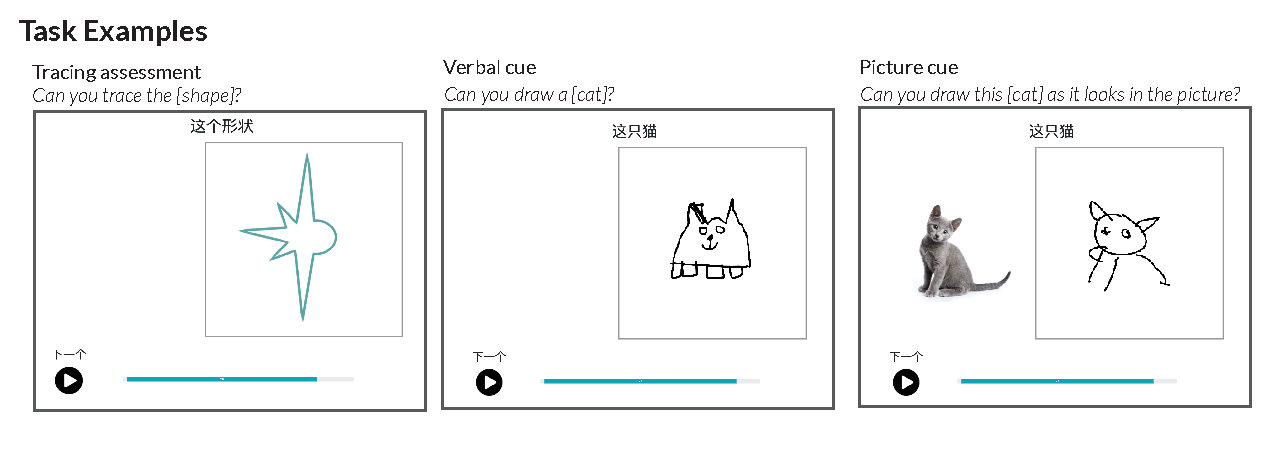
\includegraphics[width=1\linewidth]{figs/task_examples} \caption{Example trials from the tracing assessment and two drawing tasks.}\label{fig:example-tasks}
\end{figure}

\hypertarget{measuring-effort-covariates}{%
\subsection{Measuring effort covariates}\label{measuring-effort-covariates}}

For each drawing trial, children had up to 30 seconds to complete their drawings with their fingers. We recorded both the final drawings and the parameters of each stroke produced by children, allowing us to estimate the amount of time children put into their drawings (e.g., end time of last stroke --- start time of first stroke). As a second measure of effort, we also counted the number of strokes that children put into a given drawing. Finally, we estimated the proportion of the drawing canvas that was filled (e.g., \enquote{ink used}) by computing the proportion of each final drawing that were non-white pixels.

\hypertarget{measuring-tracing-accuracy}{%
\subsection{Measuring Tracing Accuracy}\label{measuring-tracing-accuracy}}

As in Long et al. (2021), we used an automated procedure for evaluating how accurately participants performed the tracing task, validated against empirical judgments of tracing quality. We decomposed tracing accuracy into two components: a shape error component and a spatial error component. Shape error reflects how closely the participant's tracing matched the contours of the target shape; the spatial error reflects how closely the location, size, and orientation of the participant's tracing matched the target shape. See Appendix for details on how these error components were computed and translated into a tracing score.

\hypertarget{measuring-drawing-recognizability}{%
\subsection{Measuring drawing recognizability}\label{measuring-drawing-recognizability}}

\hypertarget{human-recognition-scores}{%
\subsubsection{Human recognition scores}\label{human-recognition-scores}}

We assessed the recognizability of each drawing via an online recognition experiment. Adult participants based in the U.S. were recruited via Prolific for a 15 minute experiment, compensated at \$14/hour, and asked to recognize a random subset of around 140 drawings that were balanced with respect to age, category, and site. Each drawing was recognized by 10 participants. Participants were shown these drawings in a random order and asked \enquote{What does this look like?}. Participants selected an answer from the twelve categories that children were prompted to draw and were encouraged to guess. No participants were excluded from analysis for missing a catch trial (a free response describing the task that were completing). These binary recognition scores were then averaged across participants to yield a recognition score for each drawing.
(e.g., recognized by 80\% of participants).

\hypertarget{automated-recognition-scores}{%
\subsubsection{Automated recognition scores}\label{automated-recognition-scores}}

We used a combination of deep CNN activations and logistic regressions to obtain automated recognition scores, as per our pre-registered protocol. To encode the high-level visual features of each sketch, we used the VGG-19 architecture (Simonyan \& Zisserman, 2014) a deep convolutional neural network pre-trained on Imagenet classification. We used model activations in the second-to-last layer of this network, which is the first fully connected layer of the network (FC6). Raw feature representations in this layer consist of flat 4096-dimensional vectors, to which we applied channel-wise normalization across all filtered drawings in the dataset. Next, we used these features to train object category decoders. We then trained a 12-way logistic classifier with L2 regularization (tolerance = .1, regularization = .1), and used this classifier to estimate the category label for each drawing in the dataset.To avoid any bias due to imbalance in the distribution of drawings over categories, we randomly under sampled such that there were an equal number of drawings for each combination of geographical site (San Jose, Beijing) and the 12 categories. No additional metadata about the age of the child who produced each sketch was provided to the decoder. This procedure was repeated for each drawing in the dataset, yielding a binary a recognition score for each drawing.

\hypertarget{statistical-models}{%
\subsection{Statistical models}\label{statistical-models}}

To assess our main hypotheses, we fit generalized linear mixed effects models to the human recognition scores to assess the factors that influenced the recognizability of the drawings that children produced. A first generalized linear mixed effect model was fit to the recognizability scores for each drawing, including fixed effects of children's age (in years), geographical site (San Jose vs.~Beijing), and drawing task (verbal cue vs.~picture cue) and the three way interaction between these key variables. We initially planned to include random slopes for the effect of drawing task on each child (as this varied within-subjects), and random slopes for the effect the full three-way interactions between task, age, and site on each category. However, models with this complicated random effects structure failed to converge, and the reported models use the maximal random effects structure that did converge -- which included random sloops for the two-way interaction between task and age on each category.

In a secondary analysis, we aimed to understand the degree to which any of the above effects were mediated by (1) children's tracing abilities and (2) the amount of effort that children expended while drawings. We thus ran the same main model while also now including fixed effects of children's estimated tracing score (see Measuring Tracing Abilities), the time children spent drawing (in seconds), the mean intensity of the drawing (i.e.~percentage of non-white pixels), and the number of strokes children used. All predictors were scaled to have a mean of 0 and a standard deviation of 1. Finally, we also assessed the degree to which tracing ability development differed by geographical site, where tracing scores were modeled as a function of age (in years), site, and their interaction, with the same random effects structure as the first model.

This analysis plan was pre-registered at \url{https://osf.io/qymjr}. While we had initially planned to use automated recognition scores as our main dependent variable, following prior work (Long et al., 2021), we found that these automated recognition scores were only modestly correlated with human recognition scores (\(r\) = 0.40, \(t\) = 22.78, p \textless{} .001); furthermore, descriptive plots of the automated recognition scores revealed a overall difference between the two drawing tasks that was not evident in the human recognition data. To be conservative, we thus fit all of our models to the human recognition data but have made all model classifications available for future research.

\hypertarget{results}{%
\section{Results}\label{results}}

\hypertarget{confirmatory-analyses}{%
\subsubsection{Confirmatory Analyses}\label{confirmatory-analyses}}

Overall, we found relative consistency in the developmental trajectory of children's drawings: Figure \ref{fig:main-results} shows the recognizability of children's drawings at each age as a function of the drawing task and the geographical site that they were located in (all model coefficients can be found in Table 1). We found steady changes in the recognizability of children's drawings across this age range, replicating prior work with an observational dataset collected at a free-standing kiosk (Long et al., 2021). Further, we found that these changes in recognizability did not depend on the drawing task children completed: children's drawings were equally recognizable when they were asked to \enquote{Draw this rabbit as it looks in the picture} versus they were simply asked \enquote{Can you draw a rabbit?}. While we anticipated that older children might produce more recognizable drawings when provided with a picture cue -- as do adults when presented with canonical photographs of object categories (Yang \& Fan, 2021) -- this was not the case. However, we did observe a main effect of geographical site: we found that children from Beijing, China overall tended to produce more recognizable drawings than children from San Jose, USA (see coefficients in Table 1). A closer look comparing the recognizability of the drawings made at children at each age and site hints that the children from Beijing, China may tend to produce more recognizable drawings earlier in development.

In a second set of analyses, we aimed to understand the nature of this difference in recognizability across sites. We initially hypothesized that any differences in the recognizability of children's drawings across sites would be mediated by the amount of effort children expended while drawing or their tracing abilities. We thus first examined how effort and tracing abilities varied across task, age, and geographical location. Figure \ref{fig:effort-covariates} shows three effort covariates - average intensity, number of strokes used, and time spent drawing -- measured for each drawing as a function of children's age, drawing task, and geographical site. Children tended to spend more time drawing provided with a picture cue and asked to draw \enquote{the {[}rabbit{]} as it looks in the picture}, and children from Beijing tended to spend more time drawing overall. In contrast, children's tracing abilities did not vary across geographical site: Figure \ref{fig:tracing} shows the average tracing score at each age at each site. While children's tracing abilities increased steadily with age, as in prior work (Long et al., 2021), children from both sites produced equally good tracings.

We then included children's average tracing scores and effort covariates measured for each drawing (average intensity, number of strokes used, and time spent drawing) as fixed effects into a second generalized linear mixed-effects model (see Statistical Models). If the amount of effort spent or children's tracing abilities accounted the differences between sites that we observed, we reasoned that we should no longer observe a main effect of geographical location on drawing recognizability. Contra this hypothesis, however, we still observed a significant effect of geographical site (see Table 2), despite the fact that individual children's tracing abilities were strong predictors of how recognizable their drawings were. In addition, the amount of time a child spent drawing was in fact a significant negative predictor of recognizability -- indicating that the amount of effort that children expended did not necessarily result in a drawing that was more recognizable to others. Thus, these results suggest that these two groups of children differ in their ability to produce recognizable drawings of object categories in a way that is not easily explainable by effort covariates or tracing abilities.

\hypertarget{exploratory-analyses}{%
\subsubsection{Exploratory Analyses}\label{exploratory-analyses}}

In a third set of exploratory analyses, we examined how the developmental trajectory of the recognizability of children's drawings differ for different object categories. Intuitively, some object categories (e.g., cat) may be easier to draw than others (e.g., watch), resulting in shallower or steeper changes in recognizability over age. However, we had no strong hypotheses about how these trajectories might additionally vary with geographical locations.

Figure \ref{fig:item-effects} shows the recognizability of children's drawings for each of the 12 categories a function of geographical location and children's age and reveal considerable variability. For example, certain categories (e.g., cats and rabbits) were overall more difficult for children to depict such that they were distinct from one another, particularly for younger children. In addition, children from Beijing produced more recognizable drawings of certain categories at all ages -- including airplanes, birds, and rabbits -- while older children from San Jose produced more recognizable drawings of bikes. Figure \ref{fig:example-drawings} shows recognizable, randomly sampled example drawings from 6-year-olds at each category, site, and condition. These exploratory analyses thus reveal systematic differences between object categories and geographical site that do not seem easily attributable to differences in effort.

\begin{figure}[H]

{\centering 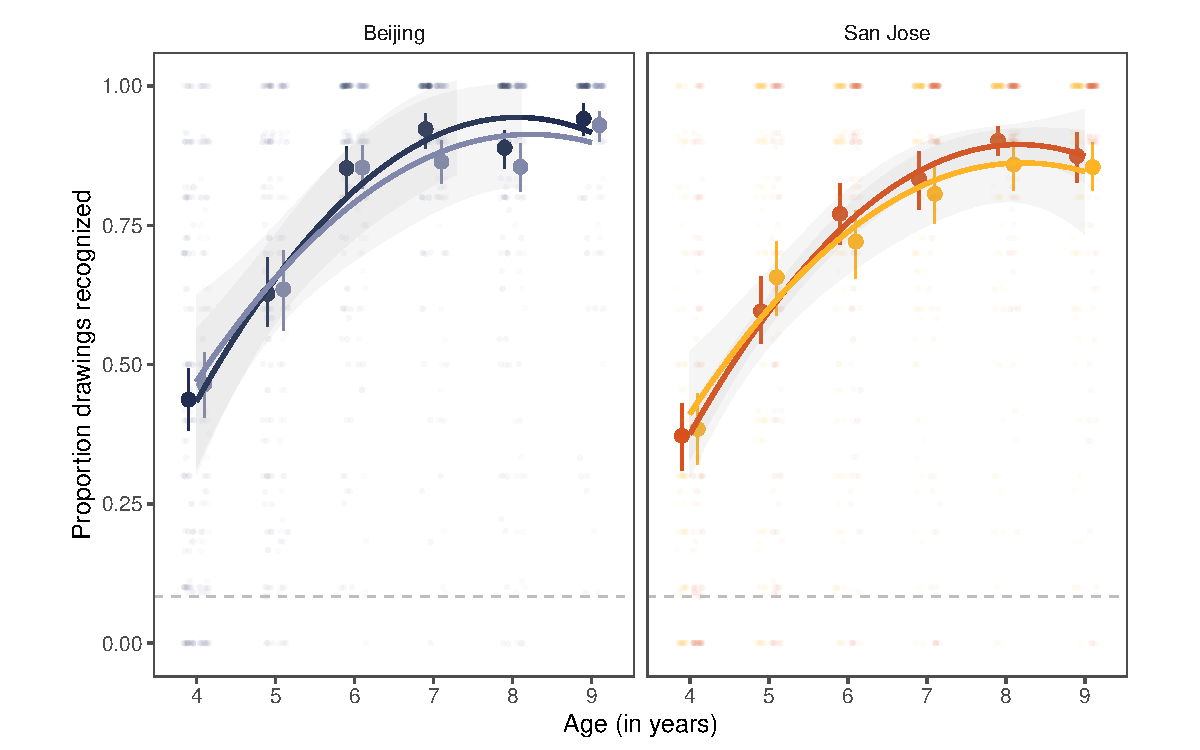
\includegraphics[width=\textwidth]{figs/main-results-1} 

}

\caption{Proportion of drawings recognized as a function of the age of the child who completed each drawing, the geographical site they were tested at (San Jose vs. Beijing), and the type of drawing task they completed. Individual data points represent drawings within each condition by an individual participant and are slightly jittered. Error bars show bootstrapped 95 percent cofnidence intervals.}\label{fig:main-results}
\end{figure}

\begin{table}[ht]
\centering
\begin{tabular}{rrrrr}
  \hline
 & Estimate & Std. Error & z value & Pr($>$$|$z$|$) \\ 
  \hline
Intercept & 1.39 & 0.16 & 8.51 & 0.000 \\ 
  Task & 0.02 & 0.26 & 0.08 & 0.936 \\ 
  Age & 1.16 & 0.14 & 8.59 & 0.000 \\ 
  Site & 0.60 & 0.16 & 3.71 & 0.000 \\ 
  Task*Age & -0.14 & 0.19 & -0.73 & 0.467 \\ 
  Task*Site & -0.19 & 0.16 & -1.17 & 0.244 \\ 
  Age*Site & 0.15 & 0.16 & 0.91 & 0.361 \\ 
  Task*Age*Site & 0.06 & 0.16 & 0.38 & 0.706 \\ 
   \hline
\end{tabular}
\caption{Model coefficients from a generalized linear mixed mode predicting the recognizability of each drawing for the main experimental contrasts.} 
\end{table}

\begin{table}[ht]
\centering
\begin{tabular}{rrrrr}
  \hline
 & Estimate & Std. Error & z value & Pr($>$$|$z$|$) \\ 
  \hline
Intercept & 1.34 & 0.15 & 8.68 & 0.000 \\ 
  Task & -0.04 & 0.26 & -0.16 & 0.873 \\ 
  Age & 0.97 & 0.14 & 7.05 & 0.000 \\ 
  Site & 0.80 & 0.16 & 5.04 & 0.000 \\ 
  Est. tracing score & 0.35 & 0.07 & 4.82 & 0.000 \\ 
  Avg. intensity & 0.06 & 0.02 & 2.47 & 0.013 \\ 
  Draw duration & -0.25 & 0.03 & -7.58 & 0.000 \\ 
  Number of strokes & 0.33 & 0.03 & 10.99 & 0.000 \\ 
  Task*Age & -0.17 & 0.19 & -0.90 & 0.370 \\ 
  Task*Site & -0.22 & 0.16 & -1.38 & 0.168 \\ 
  Age*Site & 0.04 & 0.16 & 0.22 & 0.823 \\ 
  Task*Age*Site & 0.07 & 0.16 & 0.43 & 0.665 \\ 
   \hline
\end{tabular}
\caption{Model coefficients from a generalized linear mixed mode predicting the recognizability of each drawing as a function the both the main experimental contrasts (task, site, and age) as well as several effort covariates and individual's estimates tracing abilities.} 
\end{table}

\begin{figure}[H]

{\centering 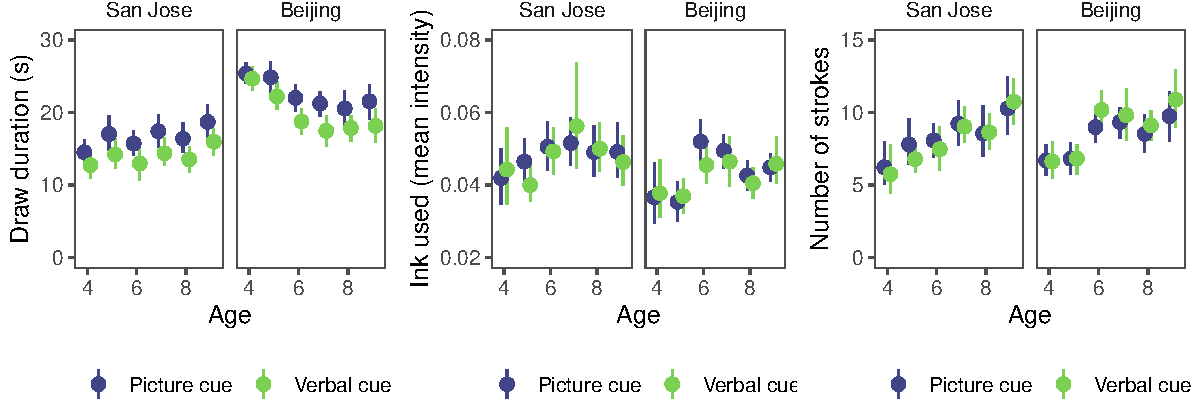
\includegraphics[width=\textwidth]{figs/effort-covariates-1} 

}

\caption{Effort covariates measured during the drawing task -- amount of time spent drawing, amount of 'ink' used, and number of strokes used -- as function of the age of the child who completed each drawing, the geographical site they were tested at (San Jose vs. Beijing), and the type of drawing task they completed. Error bars show bootstrapped 95 percent cofnidence intervals.}\label{fig:effort-covariates}
\end{figure}

\begin{figure}[H]

{\centering 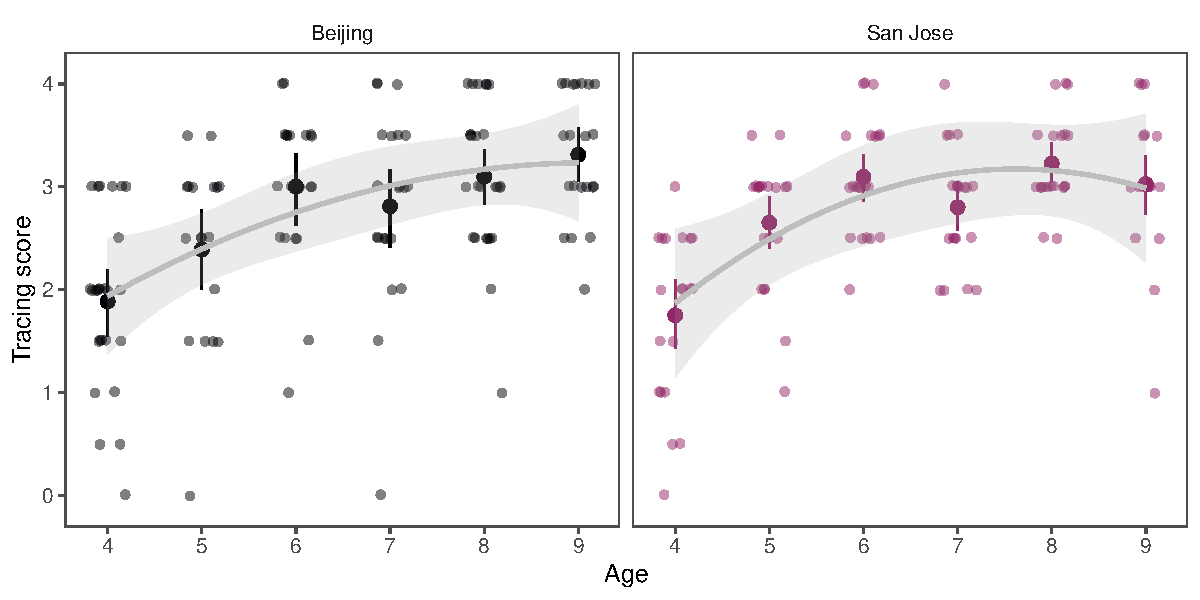
\includegraphics[width=\textwidth]{figs/tracing-1} 

}

\caption{Average tracing scores across age and site; each dot represents an average tracing score obtained for each participant and are slightly jittered. Error bars represent bootstrapped 95 percent confidence intervals.}\label{fig:tracing}
\end{figure}

\begin{figure}[H]
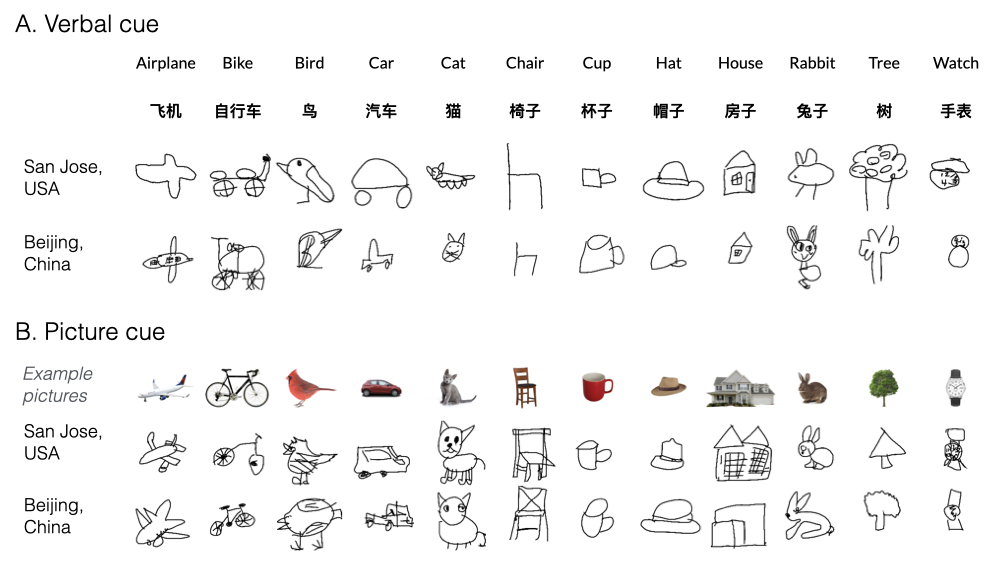
\includegraphics[width=1\linewidth]{figs/example_drawings} \caption{Randomly sampled, highly recognized drawings for each task, category, and geographical site made by 6-year-old children.}\label{fig:example-drawings}
\end{figure}

\begin{figure}[H]

{\centering 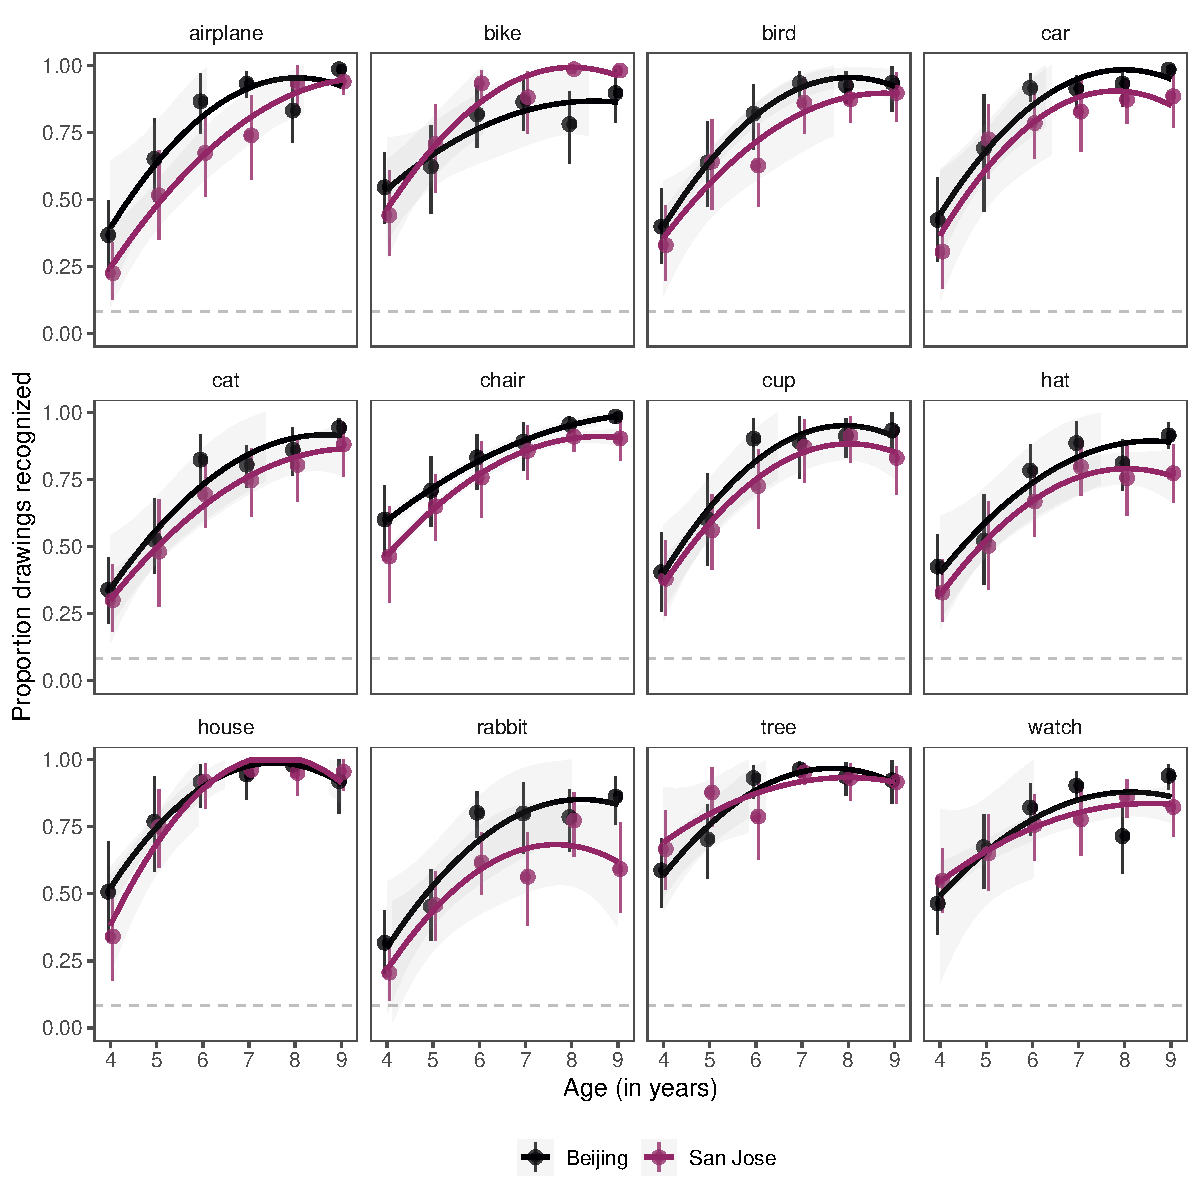
\includegraphics[width=\textwidth]{figs/item-effects-1} 

}

\caption{Developmental trajectory of drawing recognizability for each category and for each geographical site. Error bars represent 95 percent bootstrapped confidence intervals.}\label{fig:item-effects}
\end{figure}

\hypertarget{general-discussion}{%
\section{General Discussion}\label{general-discussion}}

Here, we examined the developmental trajectory of the recognizability of children's drawings across two different drawing tasks and geographical locations. Overall, we found a consistent developmental trajectory from 4-9 years of age, replicating previous work using observational datasets (Long et al., 2021). We found that asking children to draw categories when provided with a verbal cue (\enquote{Can you draw a {[}cat{]}?}) vs.~a picture cue (\enquote{Can you draw this {[}cat{]} as it looks in the picture?}) had little effect on the recognizability of the drawings that children produced. While older children may have integrated specific visual information that was present in the photographs, in keeping with prior work (Bremner \& Moore, 1984), this did not seem to change how recognizable their drawings were to outside observers. Thus, these results suggest that younger children's drawings are unlikely to be constrained by their ability to recall specific, canonical exemplars of object categories when they are trying to draw them.

Instead, we found that the recognizability of children's drawings differed between our two different geographical sites -- Beijing, China and San Jose, USA Why might this be the case? Our initial hypothesis was that children who had daily practice with a non-orthographic, complex writing system would exhibit greater dexterity in our tracing assessment task -- and that this dexterity could be a factor in how recognizable their drawings were. However, children across the two sites showed equivalent shape tracing abilities, despite the fact that children's individual tracing scores were strong predictors of the recognizability of the drawings that they produced. A second possibility is that children from preschools near Beijing were simply more engaged with the task than children recruited at a children's museum outside San Jose, USA: A more academic context could have created an environment in which children felt particularily incentivized to spend more effort on their drawings. Nonetheless, our measures of drawing's effort (e.g., amount of time spent drawing, number of strokes made) did not account for differences in recognizability across sites. Furthermore, we saw systematic differences in the object categories that were more or less recognizable across sites, which is not well-explained by this account. Thus, this finding both confirms the idea that children's visuomotor abilities strongly influence th recognizability of the drawings they produce, yet further suggests that it is far from the only factor that does so.

However, while many have sought to examine variation across different cultural contexts in children's drawings (Winner, 1989) or cognitive abilities that may be relevant to children's drawing abilities -- including object recognition (Kuwabara \& Smith, 2016) -- we note that this is there is substantial variation within different geographical locations and countries that often goes unmeasured (Amir \& McAuliffe, 2020). Indeed, this unmeasured variation within sites may lead to the low replicability of some cross-cultural findings (Carstensen, Cao, Gao, \& Frank, 2021). For example, some work has suggested that the distinction between wheat vs.~rice farming traditions explains substantial variation in cultural practices within China (Talhelm et al., 2014). We thus caution against a strong interpretation of the observed site differences, as we believe that drawings from children within the same country -- or even area code -- may differ in the very same ways children's drawings differed in this dataset. For example, the children we recruited from Beijing vs.~San Jose could differ widely in the amount of time they spending practicing drawing. If so, then children who spend more time drawing may simply have more experience communicating about the diagnostic features of different object categories.

Furthermore, we note that while this work moves beyond investigating the drawings of children at a single geographical location, these children are still in many ways non-representative of the general population. For example, children in more rural populations may spend considerably less time both consuming and producing drawings of object categories. Thus, these developmental trajectories could thus vary in several ways that are not captured by the populations represented in the the present dataset.

Indeed, a natural question for future work concerns the relationship between the degree to which children with difference kinds of experience might also show differences in their ability to produce or recognize drawings of object categories. In a U.S. based sample, prior work found that older children not only produce more recognizable drawings of object categories but tend to be better skilled at recognizing other children's drawings (Long et al., 2021). Thus, if children in different environmental contexts tend to spend more time practicing drawing, these children may also be more skilled at recognizing drawings of object categories and perhaps explicitly identifying the distinctive visual features of these categories.

Of course, these results of course do not preclude the possibility that children's drawings differed across these two conditions or geographical sites in other interesting ways beyond their recognizability. Some work has shown that young children across different cultural contexts tend to produce different tadpole drawings of varying heights and with different amounts of detail (Gernhardt, Rübeling, \& Keller, 2015) and place a horizon line in systematically different locations when drawing scenes (Senzaki, Masuda, \& Nand, 2014). Thus, finer-grained measurements of these drawings could reveal differences -- with respect to the exact visual features that children chose to include, the strategies they employed while drawing, or the order in which they chose to draw certain elements of these categories. We have thus made this dataset and the resulting code publicly available for these exploratory analyses.

Nonetheless, these results take a first step towards characterizing the consistency in the developmental trajectory of children's drawings. We propose that the systematic collection of digital drawings from children with a wide variety of experiences will help uncover the myriad factors that drive the developmental changes in children's drawings -- and in turn help us understand how different cognitive systems coordinate to produce this complex behavior.

\hypertarget{acknowledgements}{%
\section{Acknowledgements}\label{acknowledgements}}

{[}BLINDED{]}

\newpage

\hypertarget{references}{%
\section{References}\label{references}}

\begingroup
\setlength{\parindent}{-0.5in}
\setlength{\leftskip}{0.5in}

\hypertarget{refs}{}
\leavevmode\hypertarget{ref-amir2020cross}{}%
Amir, D., \& McAuliffe, K. (2020). Cross-cultural, developmental psychology: Integrating approaches and key insights. \emph{Evolution and Human Behavior}, \emph{41}(5), 430--444.

\leavevmode\hypertarget{ref-barrett1976symbolism}{}%
Barrett, M., \& Light, P. (1976). Symbolism and intellectual realism in children's drawings. \emph{British Journal of Educational Psychology}, \emph{46}(2), 198--202.

\leavevmode\hypertarget{ref-bloom1998intention}{}%
Bloom, P., \& Markson, L. (1998). Intention and analogy in children's naming of pictorial representations. \emph{Psychological Science}, \emph{9}(3), 200--204.

\leavevmode\hypertarget{ref-bremmer1984prior}{}%
Bremner, J. G., \& Moore, S. (1984). Prior visual inspection and object naming: Two factors that enhance hidden feature inclusion in young children's drawings. \emph{British Journal of Developmental Psychology}, \emph{2}(4), 371--376.

\leavevmode\hypertarget{ref-carstensen2021investigating}{}%
Carstensen, A., Cao, A., Gao, S., \& Frank, M. C. (2021). Investigating cross-cultural differences in reasoning, vision, and social cognition through replication. In \emph{Proceedings of the annual meeting of the cognitive science society} (Vol. 43).

\leavevmode\hypertarget{ref-cohn2012explaining}{}%
Cohn, N. (2012). Explaining ``i can't draw'': Parallels between the structure and development of language and drawing. \emph{Human Development}, \emph{55}(4), 167--192.

\leavevmode\hypertarget{ref-dekker2011dorsal}{}%
Dekker, T., Mareschal, D., Sereno, M. I., \& Johnson, M. H. (2011). Dorsal and ventral stream activation and object recognition performance in school-age children. \emph{NeuroImage}, \emph{57}(3), 659--670.

\leavevmode\hypertarget{ref-fan2020relating}{}%
Fan, J. E., Wammes, J. D., Gunn, J. B., Yamins, D. L., Norman, K. A., \& Turk-Browne, N. B. (2020). Relating visual production and recognition of objects in human visual cortex. \emph{Journal of Neuroscience}, \emph{40}(8), 1710--1721.

\leavevmode\hypertarget{ref-freeman1987current}{}%
Freeman, N. H. (1987). Current problems in the development of representational picture-production. \emph{Archives de Psychologie}.

\leavevmode\hypertarget{ref-fury1997children}{}%
Fury, G., Carlson, E. A., \& Sroufe, A. (1997). Children's representations of attachment relationships in family drawings. \emph{Child Development}, \emph{68}(6), 1154--1164.

\leavevmode\hypertarget{ref-gernhardt2015cultural}{}%
Gernhardt, A., Rübeling, H., \& Keller, H. (2015). Cultural perspectives on children's tadpole drawings: At the interface between representation and production. \emph{Frontiers in Psychology}, \emph{6}, 812.

\leavevmode\hypertarget{ref-hoffmann2018u}{}%
Hoffmann, D. L., Standish, C. D., Garcia-Diez, M., Pettitt, P. B., Milton, J., Zilhão, J., \ldots{} others. (2018). U-th dating of carbonate crusts reveals neandertal origin of iberian cave art. \emph{Science}, \emph{359}(6378), 912--915.

\leavevmode\hypertarget{ref-huntsinger2011cultural}{}%
Huntsinger, C. S., Jose, P. E., Krieg, D. B., \& Luo, Z. (2011). Cultural differences in chinese american and european american children's drawing skills over time. \emph{Early Childhood Research Quarterly}, \emph{26}(1), 134--145.

\leavevmode\hypertarget{ref-karmiloff1990constraints}{}%
Karmiloff-Smith, A. (1990). Constraints on representational change: Evidence from children's drawing. \emph{Cognition}, \emph{34}(1), 57--83.

\leavevmode\hypertarget{ref-kellogg1969analyzing}{}%
Kellogg, R. (1969). \emph{Analyzing children's art}. National Press Books Palo Alto, CA.

\leavevmode\hypertarget{ref-kuwabara2016cultural}{}%
Kuwabara, M., \& Smith, L. B. (2016). Cultural differences in visual object recognition in 3-year-old children. \emph{Journal of Experimental Child Psychology}, \emph{147}, 22--38.

\leavevmode\hypertarget{ref-la2001children}{}%
La Voy, S. K., Pedersen, W. C., Reitz, J. M., Brauch, A. A., Luxenberg, T. M., \& Nofsinger, C. C. (2001). Children's drawings: A cross-cultural analysis from japan and the united states. \emph{School Psychology International}, \emph{22}(1), 53--63.

\leavevmode\hypertarget{ref-light1983effects}{}%
Light, P., \& Simmons, B. (1983). The effects of a communication task upon the representation of depth relationships in young children's drawings. \emph{Journal of Experimental Child Psychology}, \emph{35}(1), 81--92.

\leavevmode\hypertarget{ref-long2021parallel}{}%
Long, B., Fan, J., Chai, Z., \& Frank, M. C. (2021). Parallel developmental changes in children's drawing and recognition of visual concepts.

\leavevmode\hypertarget{ref-long2018drawings}{}%
Long, B., Fan, J., \& Frank, M. C. (2018). Drawings as a window into developmental changes in object representations. In \emph{Proceedings of the 40th annual meeting of the cognitive science society}.

\leavevmode\hypertarget{ref-minsky1972artificial}{}%
Minsky, M., \& Papert, S. (1972). \emph{Artificial intelligence progress report}. Cambridge, MA, USA: Massachusetts Institute of Technology.

\leavevmode\hypertarget{ref-natu2016development}{}%
Natu, V. S., Barnett, M. A., Hartley, J., Gomez, J., Stigliani, A., \& Grill-Spector, K. (2016). Development of neural sensitivity to face identity correlates with perceptual discriminability. \emph{Journal of Neuroscience}, \emph{36}(42), 10893--10907.

\leavevmode\hypertarget{ref-pailian2016visual}{}%
Pailian, H., Libertus, M. E., Feigenson, L., \& Halberda, J. (2016). Visual working memory capacity increases between ages 3 and 8 years, controlling for gains in attention, perception, and executive control. \emph{Attention, Perception, \& Psychophysics}, \emph{78}(6), 1556--1573.

\leavevmode\hypertarget{ref-piaget1929child}{}%
Piaget, J. (1929). The child's concept of the world. \emph{Londres, Routldge \& Kegan Paul}.

\leavevmode\hypertarget{ref-rehrig2018does}{}%
Rehrig, G., \& Stromswold, K. (2018). What does the dap: IQ measure?: Drawing comparisons between drawing performance and developmental assessments. \emph{The Journal of Genetic Psychology}, \emph{179}(1), 9--18.

\leavevmode\hypertarget{ref-senzaki2014holistic}{}%
Senzaki, S., Masuda, T., \& Nand, K. (2014). Holistic versus analytic expressions in artworks: Cross-cultural differences and similarities in drawings and collages by canadian and japanese school-age children. \emph{Journal of Cross-Cultural Psychology}, \emph{45}(8), 1297--1316.

\leavevmode\hypertarget{ref-simonyan2014very}{}%
Simonyan, K., \& Zisserman, A. (2014). Very deep convolutional networks for large-scale image recognition. \emph{arXiv Preprint arXiv:1409.1556}.

\leavevmode\hypertarget{ref-sitton1992drawing}{}%
Sitton, R., \& Light, P. (1992). Drawing to differentiate: Flexibility in young children's human figure drawings. \emph{British Journal of Developmental Psychology}, \emph{10}(1), 25--33.

\leavevmode\hypertarget{ref-talhelm2014large}{}%
Talhelm, T., Zhang, X., Oishi, S., Shimin, C., Duan, D., Lan, X., \& Kitayama, S. (2014). Large-scale psychological differences within china explained by rice versus wheat agriculture. \emph{Science}, \emph{344}(6184), 603--608.

\leavevmode\hypertarget{ref-willats2006making}{}%
Willats, J. (2006). \emph{Making sense of children's drawings}. Psychology Press.

\leavevmode\hypertarget{ref-winner1989can}{}%
Winner, E. (1989). How can chinese children draw so well? \emph{Journal of Aesthetic Education}, \emph{23}(1), 41--63.

\leavevmode\hypertarget{ref-yang2021visual}{}%
Yang, J., \& Fan, J. E. (2021). Visual communication of object concepts at different levels of abstraction. \emph{arXiv Preprint arXiv:2106.02775}.

\endgroup

\end{document}
